\documentclass[12pt]{article}

% basic package list
\usepackage[T1]{fontenc}
\usepackage{fontspec}
\defaultfontfeatures{Mapping=tex-text}
\usepackage[margin=25mm]{geometry}
\usepackage{amsmath}
\usepackage{amsfonts}
\usepackage{amssymb}
\usepackage{graphicx}
%\setmainfont{???}

% other packages
\usepackage{xunicode}
\usepackage{xltxtra}
\usepackage{hyperref}         % hyperlinks
\usepackage{booktabs}         % professional-quality tables
\usepackage{url}              % simple URL typesetting
\usepackage{natbib}
\usepackage[modulo]{lineno}
\usepackage{sectsty}          % to change section font size
\usepackage{mathtools}

% set additional parameters
\setcitestyle{authoryear,open={(},close={)}}
\graphicspath {{Figures/}}

\sectionfont{\fontsize{18}{22}\selectfont}
\subsectionfont{\fontsize{16}{19}\selectfont}

\renewcommand{\thefigure}{S\arabic{figure}}

\setcounter{figure}{0}

\title{Supporting Information for: Joint inference of adaptive and demographic history from temporal population genomic data}
\author{Vitor A. C. Pavinato$^1$, Stéphane de Mita$^2$, Jean-Michel Marin$^3$, \\
			Miguel Navascués$^1$$^*$}
\font\myfont=cmr12 at 10pt
\date{{\myfont %
    $^1$UMR Centre de Biologie pour la Gestion des Populations, INRAE, France\\%
    $^2$UMR Interactions Arbres-Microorganismes, INRAE, France \\%
    $^3$UMR Institut Montpelliérain Alexander Grothendieck, Université de Montpellier, France\\%
    $^*$corresponding author: miguel.navascues@inra.fr\\[2ex]%
    }
    \today    
}
\begin{document}
\maketitle
\newpage
\section*{S1 Supplementary Methods}

\subsection*{S1.1 Model}

A schematic representation of the model used to simulate temporal population genomics data is presented in figure S1. The model was composed by two periods: 1) the burn-in period (period 1 in the main text) and 2) the sampling period (period 2 in the main text). Both periods had independent prior for the population census size: $N_{cs1}$ and $N_{cs2}$. Since our interest were in how demography and the selection affect affect each other in between the period of the samples of individuals, the summary statistics were calculated with the genotypic data sampled in each time-points, at TS1 and TS2, apart $\tau$ generations. In order to simulate the dynamic of selection acting on the genome, we divided the genome of each diploid individual in "neutral" and "non-neutral"regions. It roughly mimic intergenic and genic regions of a genome. We simplified in this because It allowed us define different prior for the number of non-neutral regions and for the number of mutations in each non-neutral regions. The proportion of non-neutral regions was defined by $P_{R}$ and the probability of a beneficial mutation to arise in a non-neutral regions was defined by $P_{B}$. The compound parameter $P_{S} = P_{R}*P_{B}$ defined the proportion of selection mutation that might arise in a simulation.

\begin{figure}[ht]
  \centering
  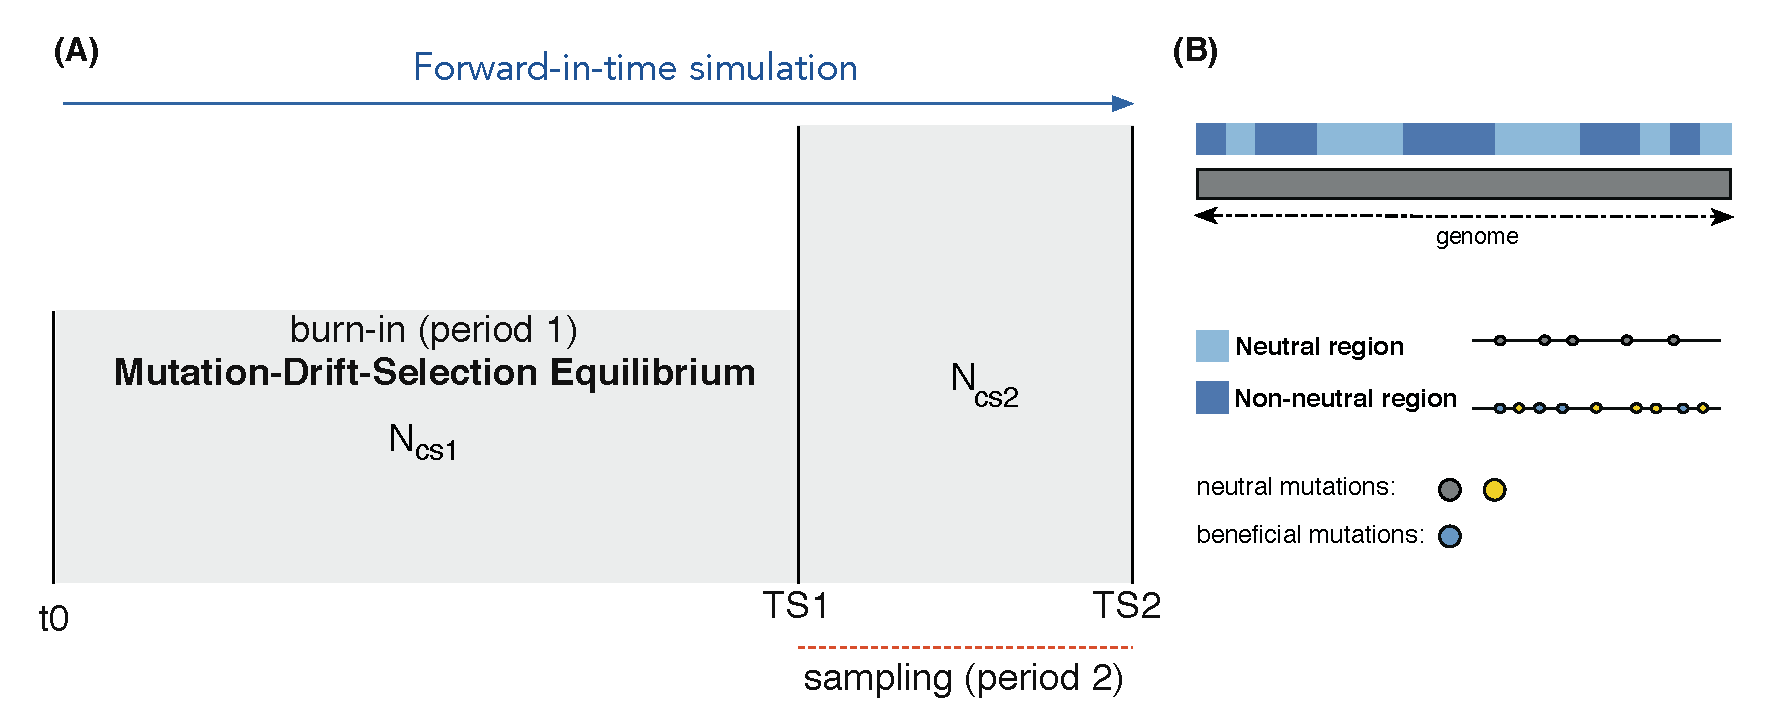
\includegraphics[width=0.95\textwidth]{Figures/model.pdf}
  \label{fig:figS1}
  \caption{A schematic representation of the model used to simulate temporal population genomics data. \textbf{(A)} the population model and \textbf{(B)} the genome model.}
\end{figure}

\subsection*{S1.2 List of summary statistics}

Below is the list of the summary statistic used to produced the reference table for the evaluation of ABC-RF:
\begin{enumerate}
	\item Locus-specific summary statistics (LSS) - SNP-based:
    \begin{enumerate}
    	\item Expected heterozygosity - $H_E$;
        \item Jost's $D$ \citep{Jost:2008cs,Jost:2009hn} - $Dj$;
        \item Weir and Cockerham's $F_{ST}$ \citep{Weir:1984dx} - $WC_{ST}$;
    \end{enumerate}
    \item Locus-specific summary statistics - window-based:
    \begin{enumerate}
        \item Number of polymorphic sites $S$;
        \item Nucleotide diversity $\pi$ \citep{Nei:1979uk};
        \item Watterson's 4Nu estimator \citep{Watterson:1975bh} - $thetaW$;
        \item Tajima's D \citep{Tajima:1989un} - $TjD$;
        \item Net distance between populations $Da$;
        \item Rozas et al.'s $ZZ$ \citep{Rozas:2001wc};
        \item Average of $R^2$ over all pairwise comparisons $Z_{nS}$ \citep{Kelly:1997uja}; 
    \end{enumerate}
    \item Global summary statistics:
    \begin{enumerate}
        \item All summary statistics enumerated above;
        \item binned Joint Site-frequency spectrum $SFS$ \citep{Ewing:2016gv};
        \item mean, variance, kurtosis, skewness and the 5\% and 95\% quantiles of all intra-locus summary statistics calculated above;
    \end{enumerate}
\end{enumerate}

\subsection*{S1.3 Code for each summary statistics}
The code for each summary statistics as they were in the reference table are presented below:

\begin{enumerate}
    \item Global summary statistics: \texttt{GSS\_He, GSS\_Dj, GSS\_WCst, GSS\_S, GSS\_thetaW, GSS\_Pi, GSS\_D, GSS\_Da, GSSp\_He1, GSSp\_He2, GSSp\_S1, GSSp\_S2, GSSp\_thetaW1, GSSp\_thetaW2, GSSp\_Pi1, GSSp\_Pi2, GSSp\_D1, GSSp\_D2};
    \item Site-frequency spectrum: \texttt{SFSbin10\_1, SFSbin10\_2, SFSbin10\_3, SFSbin10\_4, SFSbin10\_5, SFSbin10\_6, SFSbin10\_7, SFSbin10\_8, SFSbin10\_9, SFSbin10\_10};
    \item Mean of LSS: \texttt{MEAN\_LSS\_He, MEAN\_LSS\_Dj, MEAN\_LSS\_WCst, MEAN\_LSSp\_He1, MEAN\_LSSp\_He2, MEAN\_WSS500\_He, MEAN\_WSS500\_Dj, MEAN\_WSS500\_WCst, MEAN\_WSS500\_S, MEAN\_WSS500\_thetaW, MEAN\_WSS500\_Pi, MEAN\_WSS500\_D, MEAN\_WSS500\_Da, MEAN\_WSSp500\_He1, MEAN\_WSSp500\_He2, MEAN\_WSSp500\_S1, MEAN\_WSSp500\_S2, MEAN\_WSSp500\_thetaW1, MEAN\_WSSp500\_thetaW2, MEAN\_WSSp500\_Pi1, MEAN\_WSSp500\_Pi2, MEAN\_WSSp500\_D1, MEAN\_WSSp500\_D2};
    \item Variance of LSS: \texttt{VAR\_LSS\_He, VAR\_LSS\_Dj, VAR\_LSS\_WCst, VAR\_LSSp\_He1, VAR\_LSSp\_He2, VAR\_WSS500\_He, VAR\_WSS500\_Dj, VAR\_WSS500\_WCst, VAR\_WSS500\_S, VAR\_WSS500\_thetaW, VAR\_WSS500\_Pi, VAR\_WSS500\_D, VAR\_WSS500\_Da, VAR\_WSSp500\_He1, VAR\_WSSp500\_He2, VAR\_WSSp500\_S1, VAR\_WSSp500\_S2, VAR\_WSSp500\_thetaW1, VAR\_WSSp500\_thetaW2, VAR\_WSSp500\_Pi1, VAR\_WSSp500\_Pi2, VAR\_WSSp500\_D1, VAR\_WSSp500\_D2};
    \item Kurtosis of LSS: \texttt{KURT\_LSS\_He, KURT\_LSS\_Dj, KURT\_LSS\_WCst, KURT\_LSSp\_He1, KURT\_LSSp\_He2, KURT\_WSS500\_He, KURT\_WSS500\_Dj, KURT\_WSS500\_WCst, KURT\_WSS500\_Pi, KURT\_WSS500\_D, KURT\_WSS500\_Da, KURT\_WSSp500\_He1, KURT\_WSSp500\_He2, KURT\_WSSp500\_S1, KURT\_WSSp500\_S2, KURT\_WSSp500\_thetaW1, KURT\_WSSp500\_thetaW2, KURT\_WSSp500\_Pi1, KURT\_WSSp500\_Pi2, KURT\_WSSp500\_D1, KURT\_WSSp500\_D2};
    \item Skewness of LSS: \texttt{SKEW\_LSS\_He, SKEW\_LSS\_Dj, SKEW\_LSS\_WCst, SKEW\_LSSp\_He1, SKEW\_LSSp\_He2, SKEW\_WSS500\_He, SKEW\_WSS500\_Dj, SKEW\_WSS500\_WCst, SKEW\_WSS500\_Pi, SKEW\_WSS500\_D, SKEW\_WSS500\_Da, SKEW\_WSSp500\_He1, SKEW\_WSSp500\_He2, SKEW\_WSSp500\_S1, SKEW\_WSSp500\_S2, SKEW\_WSSp500\_thetaW1, SKEW\_WSSp500\_thetaW2, SKEW\_WSSp500\_Pi1, SKEW\_WSSp500\_Pi2, SKEW\_WSSp500\_D1, SKEW\_WSSp500\_D2};
    \item 5\% quantile of LSS: \texttt{Q05\_LSS\_He, Q05\_LSS\_Dj, Q05\_LSS\_WCst, Q05\_LSSp\_He1,  Q05\_LSSp\_He2, Q05\_WSS500\_He, Q05\_WSS500\_Dj, Q05\_WSS500\_WCst, Q05\_WSS500\_S,         Q05\_WSS500\_thetaW, Q05\_WSS500\_Pi, Q05\_WSS500\_D, Q05\_WSS500\_Da, Q05\_WSSp500\_He1,     Q05\_WSSp500\_He2, Q05\_WSSp500\_S1, Q05\_WSSp500\_S2, Q05\_WSSp500\_thetaW1, Q05\_WSSp500\_thetaW2, Q05\_WSSp500\_Pi1, Q05\_WSSp500\_Pi2, Q05\_WSSp500\_D1, Q05\_WSSp500\_D2};
    \item 95 \% quantile of LSS: \texttt{Q95\_LSS\_He,Q95\_LSS\_Dj, Q95\_LSS\_WCst, Q95\_LSSp\_He1, Q95\_LSSp\_He2, Q95\_WSS500\_He,Q95\_WSS500\_Dj, Q95\_WSS500\_WCst, Q95\_WSS500\_S, Q95\_WSS500\_thetaW, Q95\_WSS500\_Pi, Q95\_WSS500\_D, Q95\_WSS500\_Da, Q95\_WSSp500\_He1, Q95\_WSSp500\_He2, Q95\_WSSp500\_S1, Q95\_WSSp500\_S2, Q95\_WSSp500\_thetaW1, Q95\_WSSp500\_thetaW2, Q95\_WSSp500\_Pi1, Q95\_WSSp500\_Pi2, Q95\_WSSp500\_D1, Q95\_WSSp500\_D2}.
\end{enumerate}

\newpage
\section*{S2 Supplementary Results}

\subsection*{S2.1 ABC Random Forests for parameter inference}
\begin{figure}[ht]
  \centering
  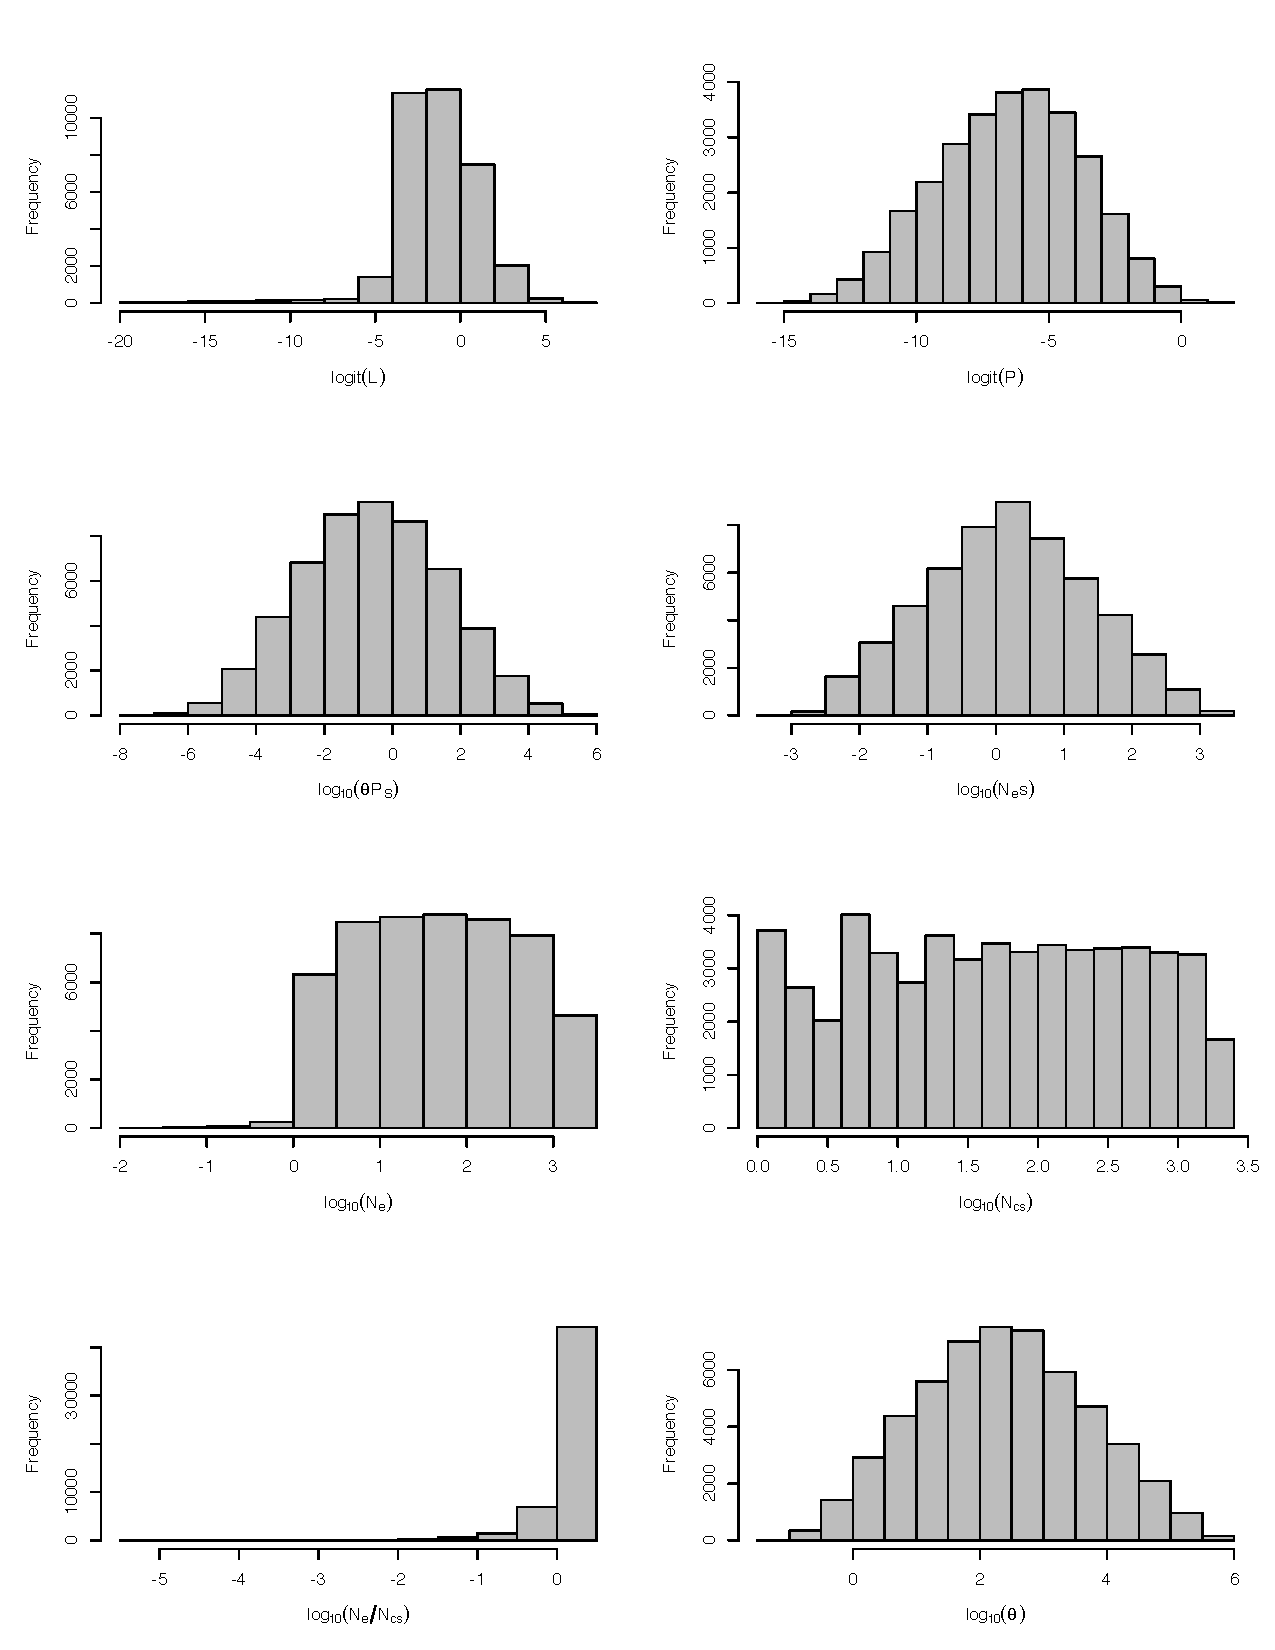
\includegraphics[width=0.75\textwidth]{Figures/parameters_histograms.pdf}
  \label{fig:figS2}
  \caption{Parameter distribution for the prior values and latent variables.}
\end{figure}

\begin{figure}[ht]
  \centering
  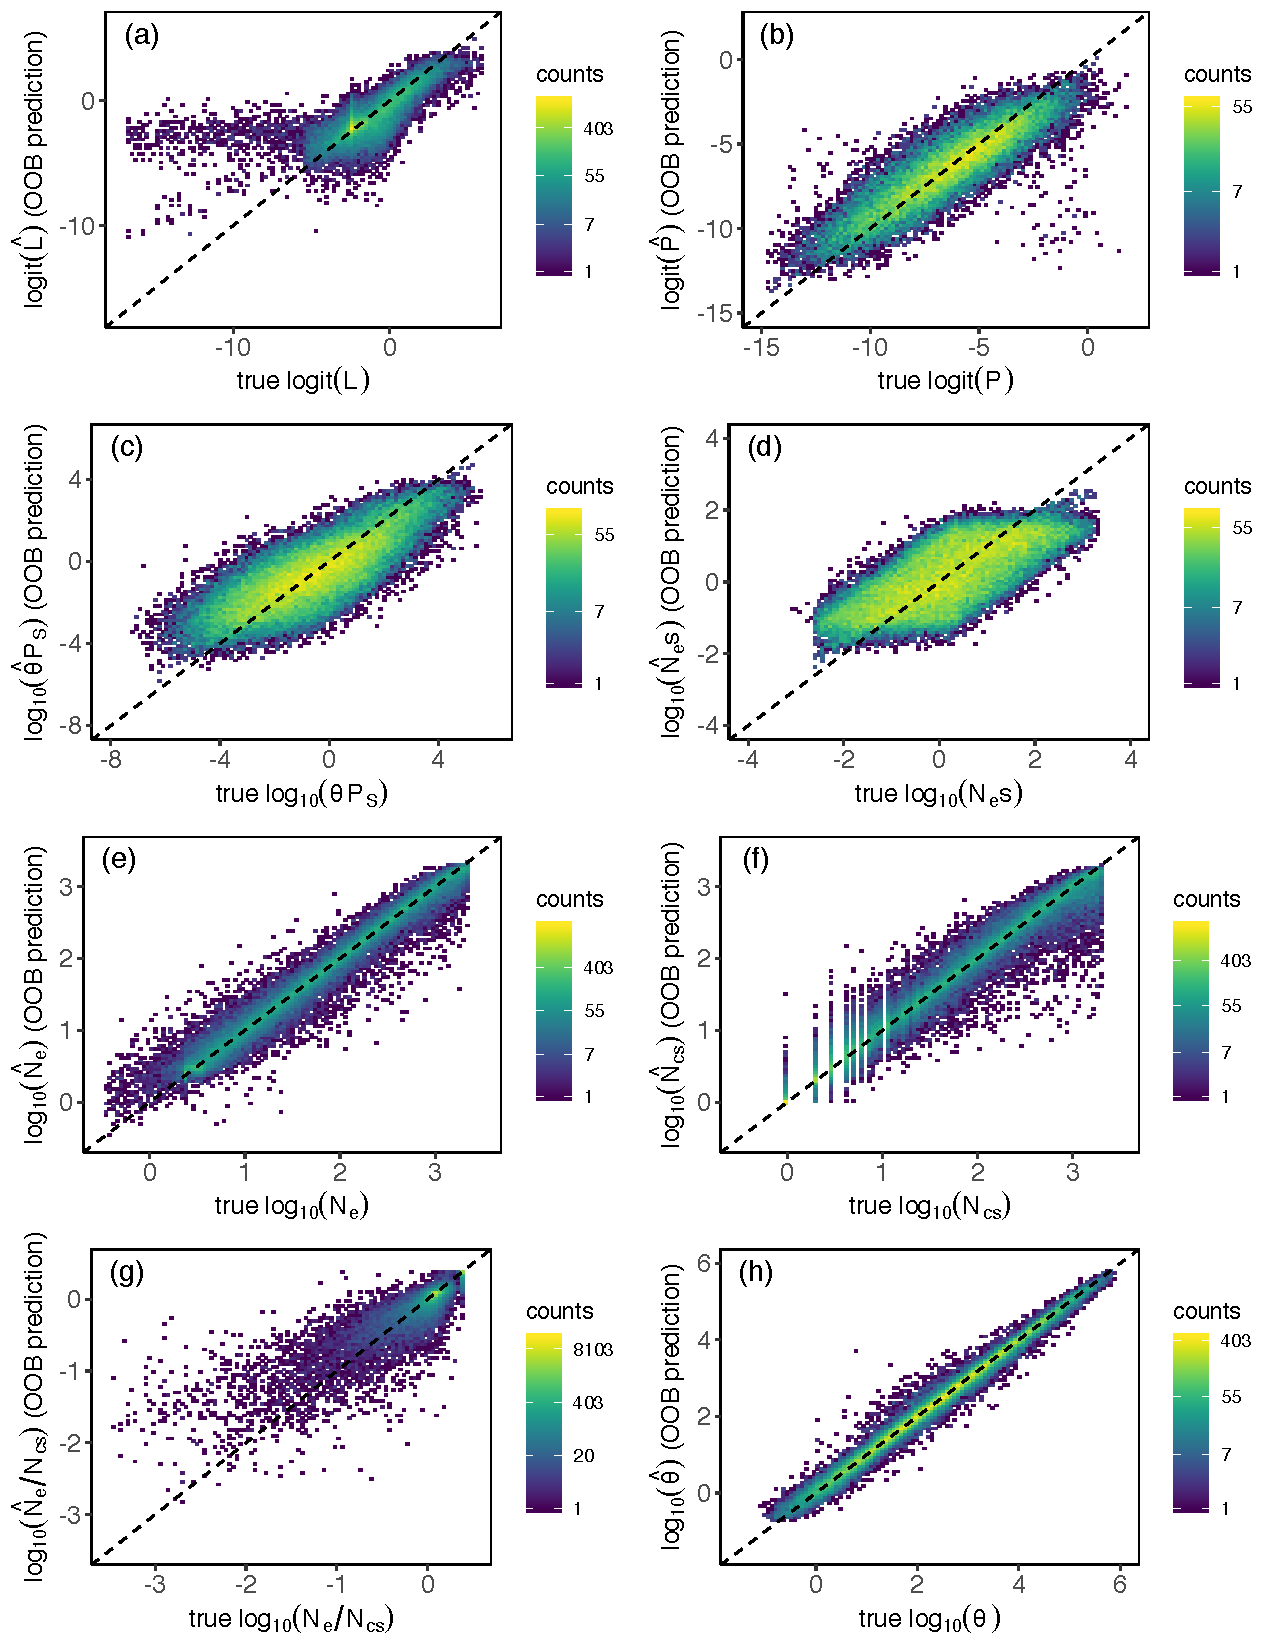
\includegraphics[width=0.80\textwidth]{Figures/oob_plots_ggplot2_mod.pdf}
  \label{fig:figS3}
  \caption{The correlation between the true value and the the value predicted by the ABC-RF for the trained Random Forests. \textbf{(a)} substitution load $L$; \textbf{(b)} proportion of strongly selected beneficial mutations $P$; \textbf{(c)} scale population size of beneficial mutation $\theta P_{\mathrm{S}}$; \textbf{(d)} overall strength of selection was calculated as $N_{\mathrm{e}}s$; \textbf{(e)} effective population size $N_{\mathrm{e}}$; \textbf{(f)} population census size $N_{\mathrm{cs}}$; \textbf{(g)} ratio between the effective size and the population census size; and \textbf{(h)} scale population size $\theta$.}
\end{figure}

\begin{figure}[ht]
  \centering
  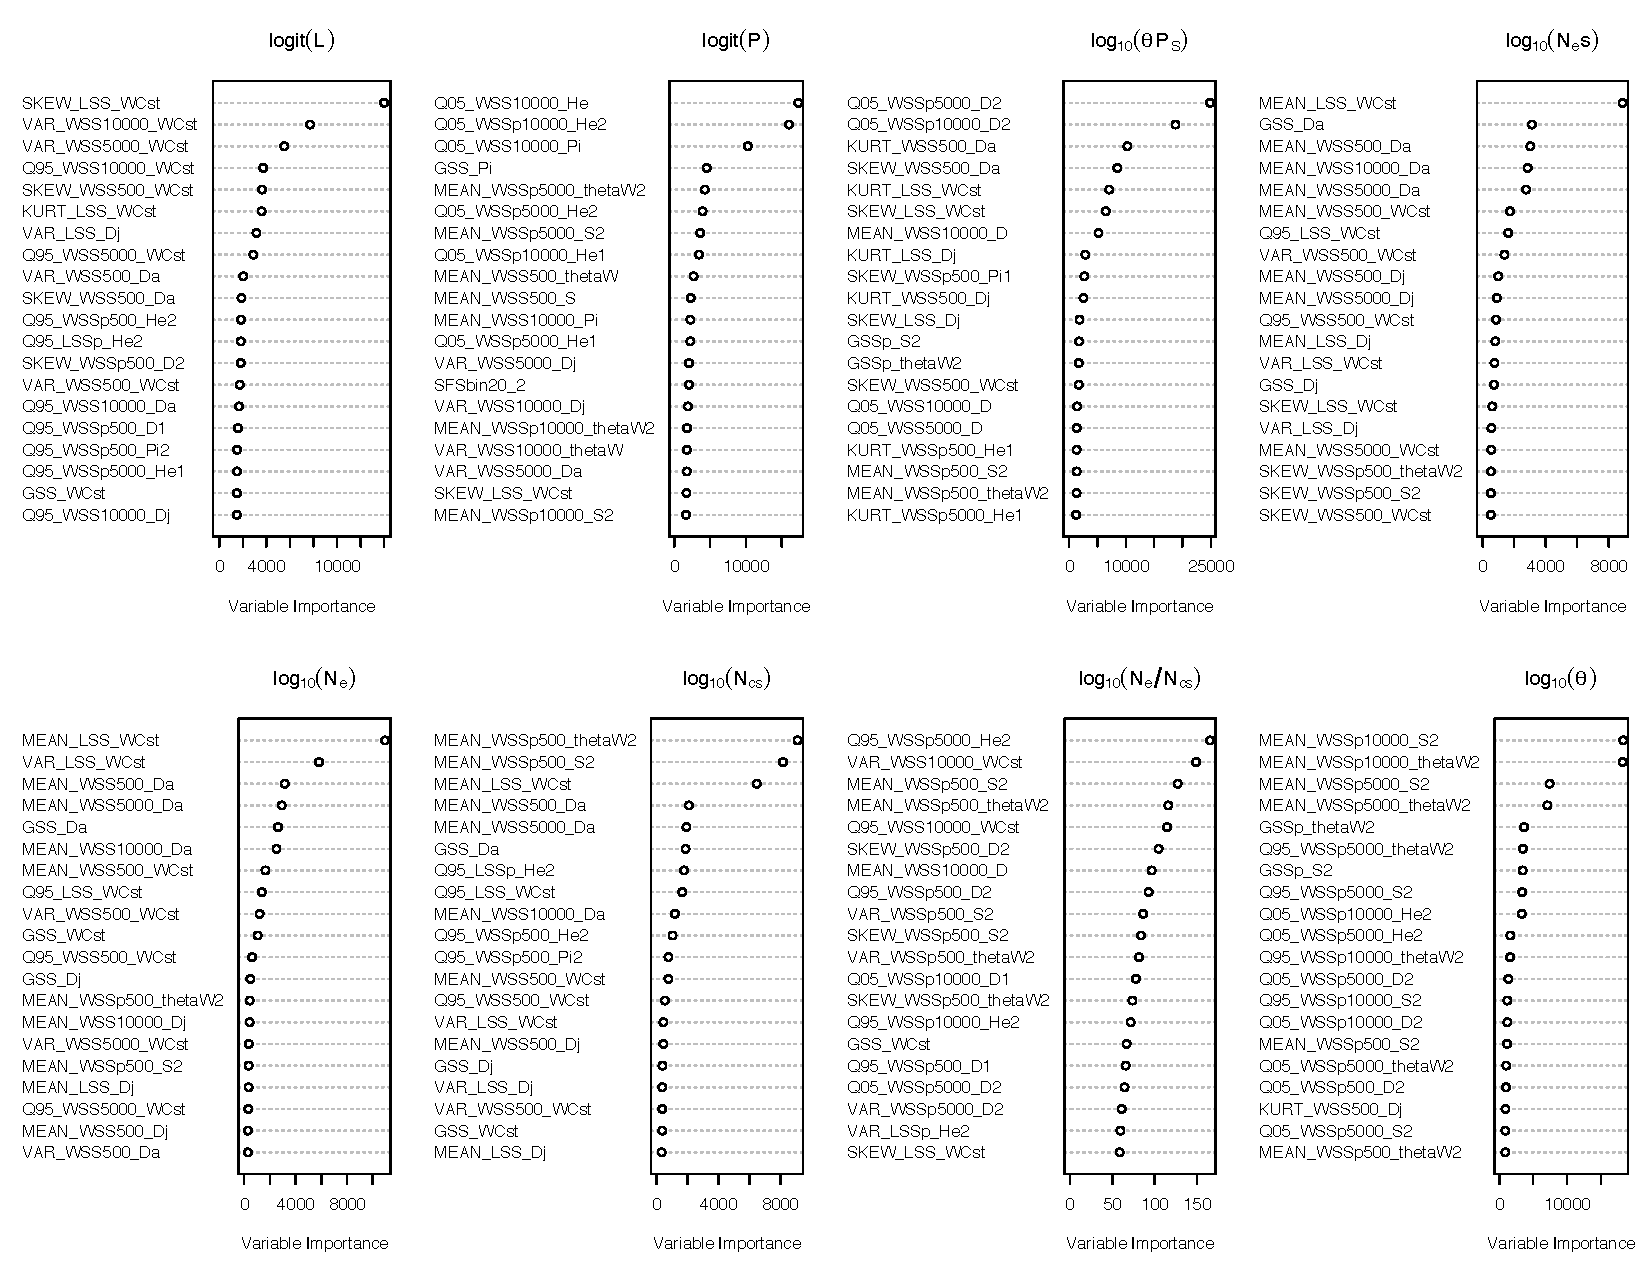
\includegraphics[width=0.9\textwidth]{Figures/varimportance_plots.pdf}
  \label{fig:figS4}
  \caption{Variance importance plots for the ABC-RF based parameter estimation.}
\end{figure}

\newpage
\subsection*{S2.1 ABC Random Forests for classification}
\begin{figure}[ht]
  \centering
  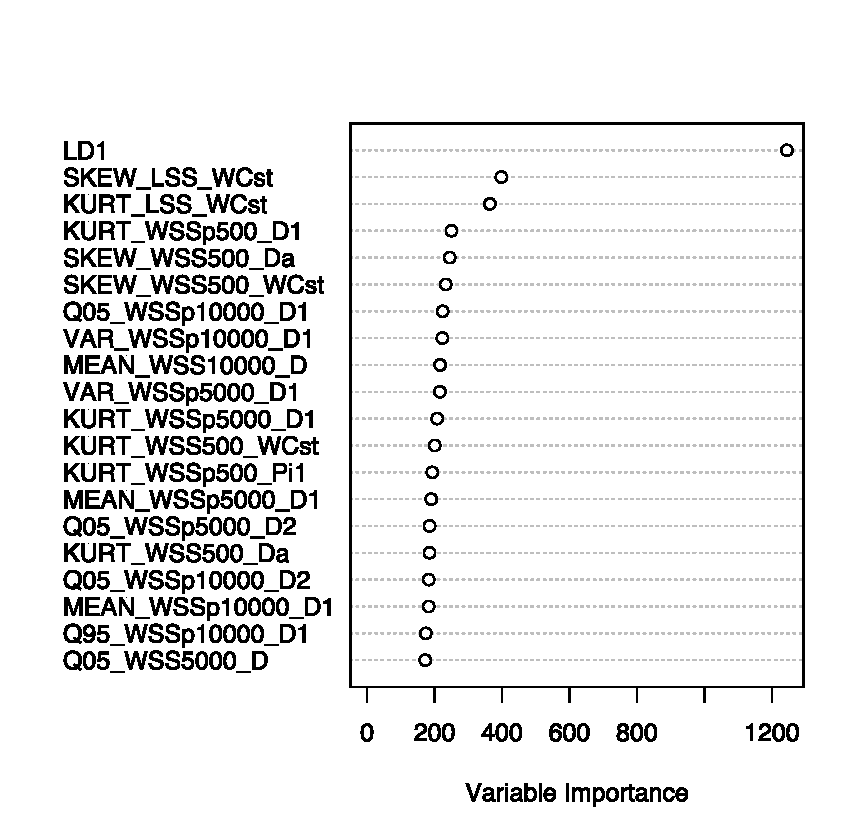
\includegraphics[width=0.65\textwidth]{Figures/varImportance_class.pdf}
  \label{fig:figS5}
  \caption{Variance importance plots for the ABC-RF based classification.}
\end{figure}

\subsubsection*{S2.1.3 Dataset}
\begin{figure}[ht]
  \centering
  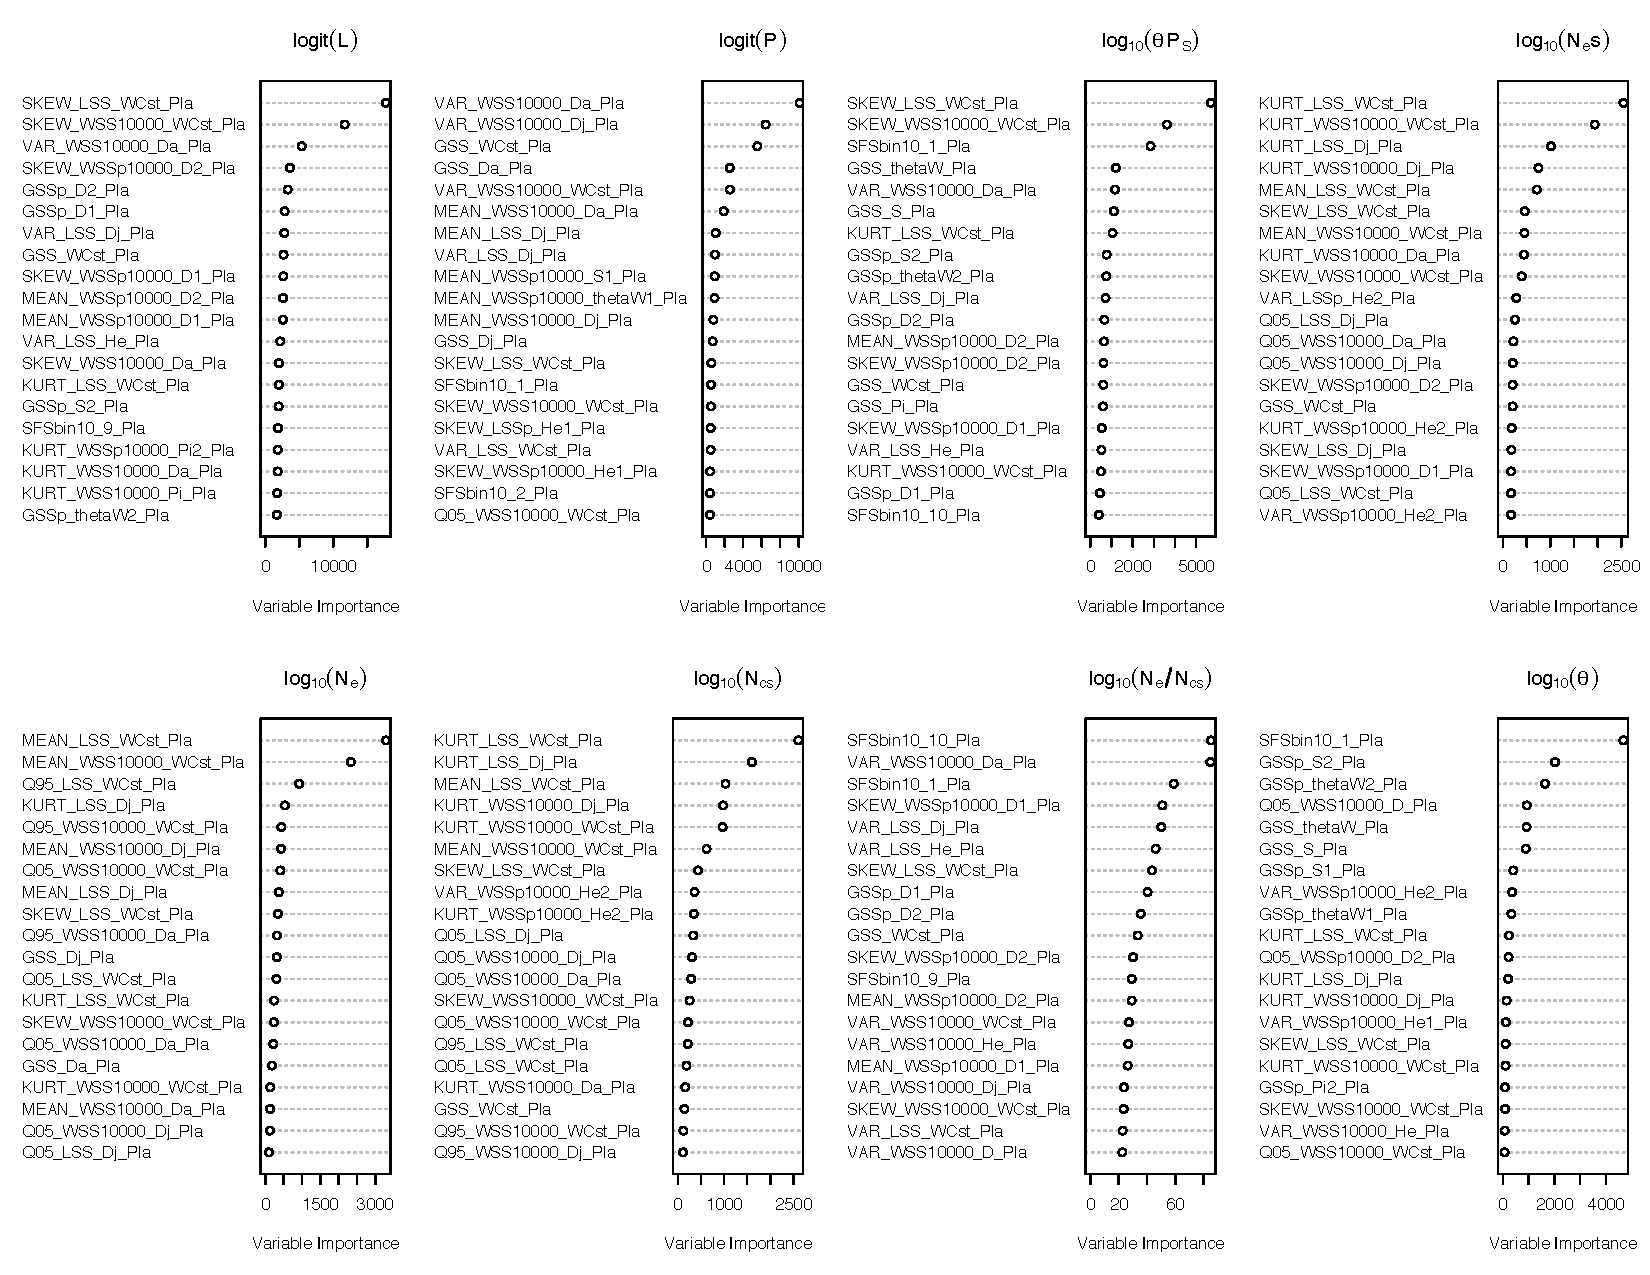
\includegraphics[width=0.9\textwidth]{Figures/varimportance_plots_placerita.pdf}
  \label{fig:figS6}
  \caption{Variance importance plots for the ABC-RF based parameter estimation.}
\end{figure}

\begin{figure}[ht]
  \centering
  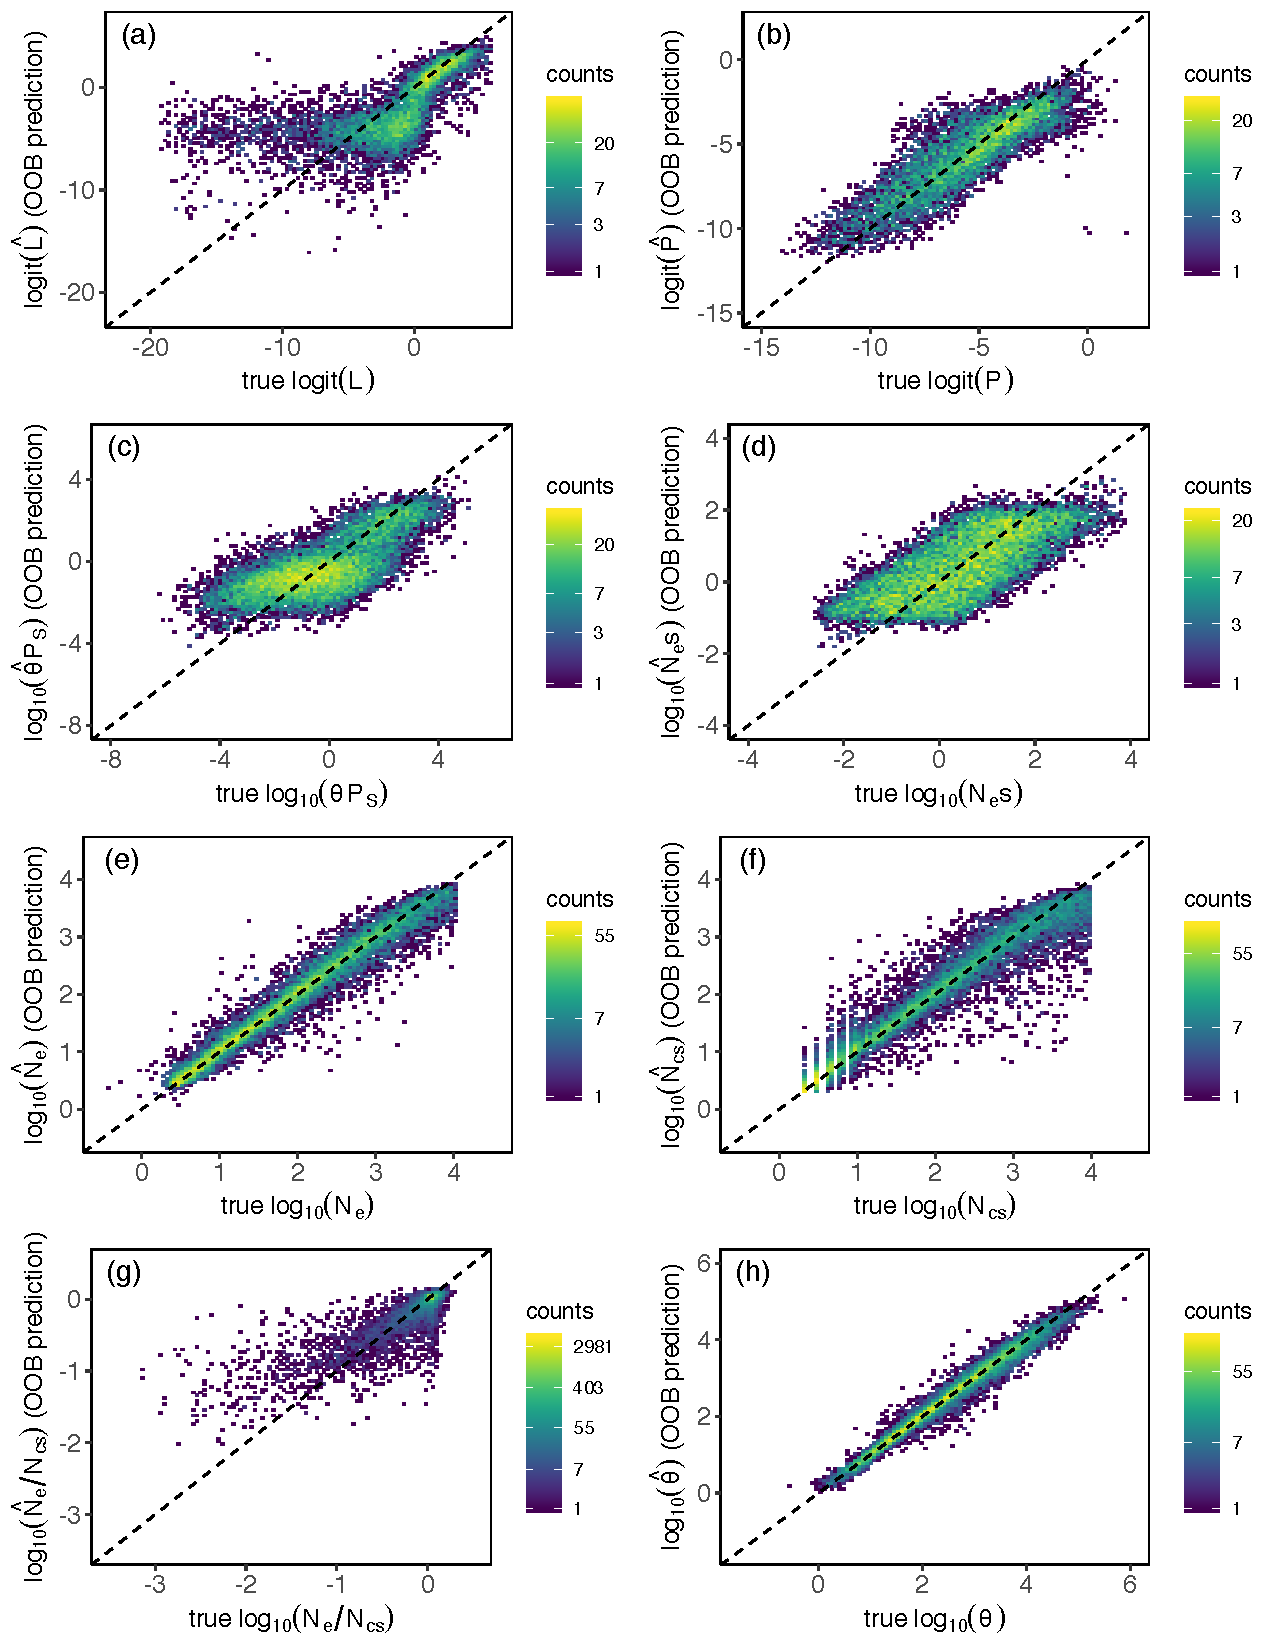
\includegraphics[width=0.95\textwidth]{Figures/oob_plots_ggplot2_placerita_mod.pdf}
  \label{fig:figS7}
  \caption{The correlation between the true value and the the value predicted by the ABC-RF.}
\end{figure}

\begin{figure}[ht]
  \centering
  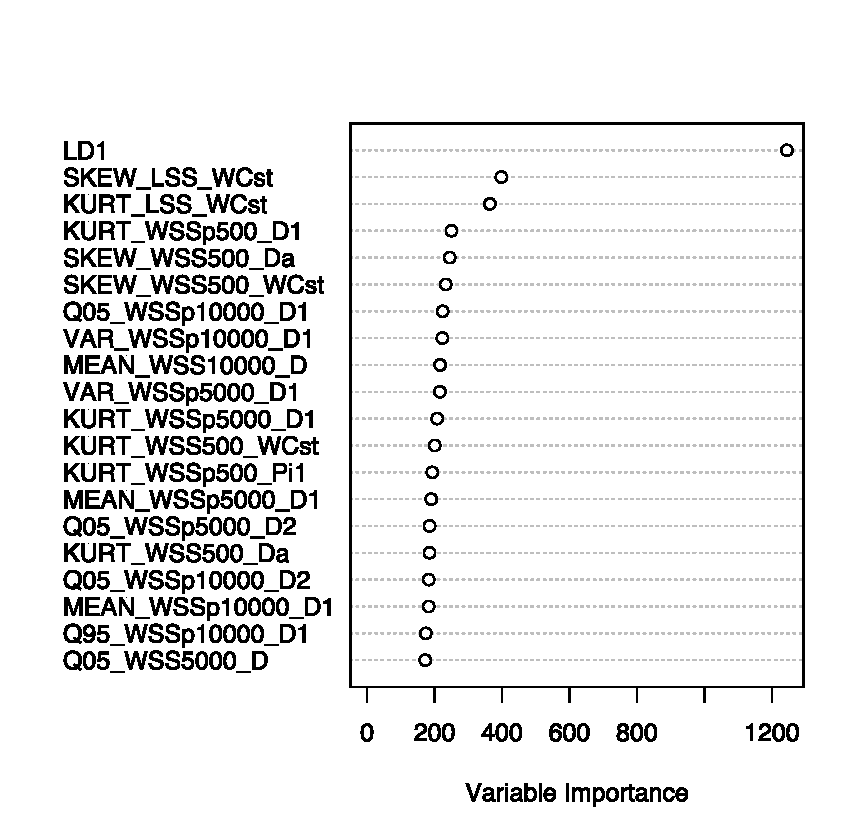
\includegraphics[width=0.75\textwidth]{Figures/varImportance_class.pdf}
  \label{fig:figS8}
  \caption{Variance importance plots for the ABC-RF based classification.}
\end{figure}

\begin{figure}[ht]
  \centering
  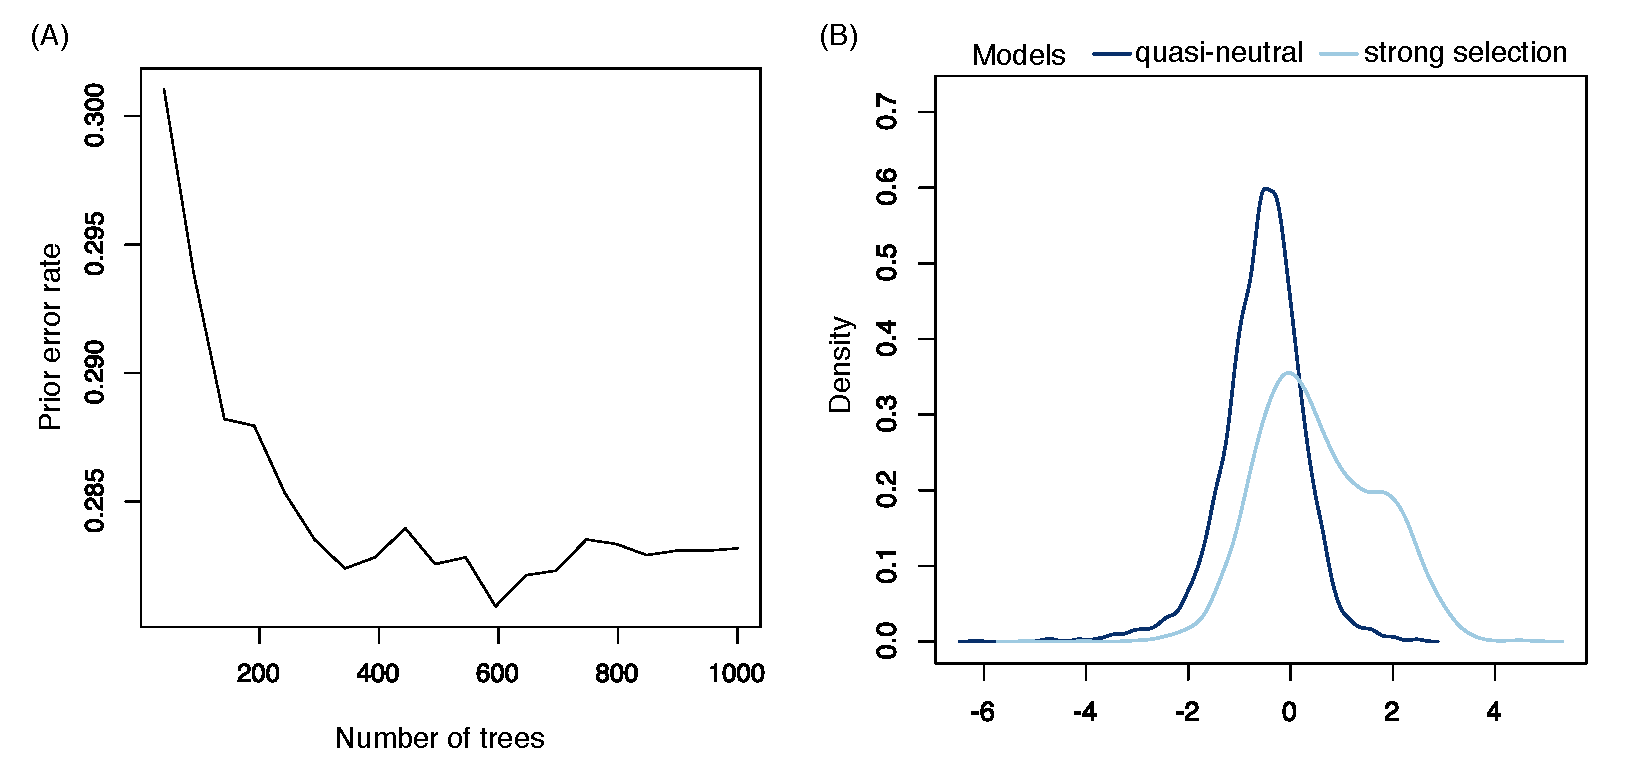
\includegraphics[width=0.95\textwidth]{Figures/lda_plot_classErr_comb_placerita.pdf}
  \label{fig:figS9}
  \caption{Classification error rate.}
\end{figure}


\newpage
\bibliographystyle{apalike}
\bibliography{references}
\end{document}
